\documentclass[tikz, border=25pt]{standalone}
\usetikzlibrary{arrows.meta, positioning, calc, fit, backgrounds}
\usepackage{moresize}
\usepackage{amssymb}

% Define custom keys for separate horizontal padding controls
\pgfkeys{
	/tikz/inner xsep-left/.store in=\innerxsepleft,
	/tikz/inner xsep-right/.store in=\innerxsepright,
	/tikz/inner xsep-left=0cm,   % Initial default
	/tikz/inner xsep-right=0cm,  % Initial default
}

% ==========================================================
% GLOBAL FONT CONFIGURATION
% ==========================================================
\newcommand{\diagramfontsize}{\fontsize{80pt}{30pt}\selectfont}
\DeclareMathSizes{80}{80}{18}{35} 

\begin{document}
	
	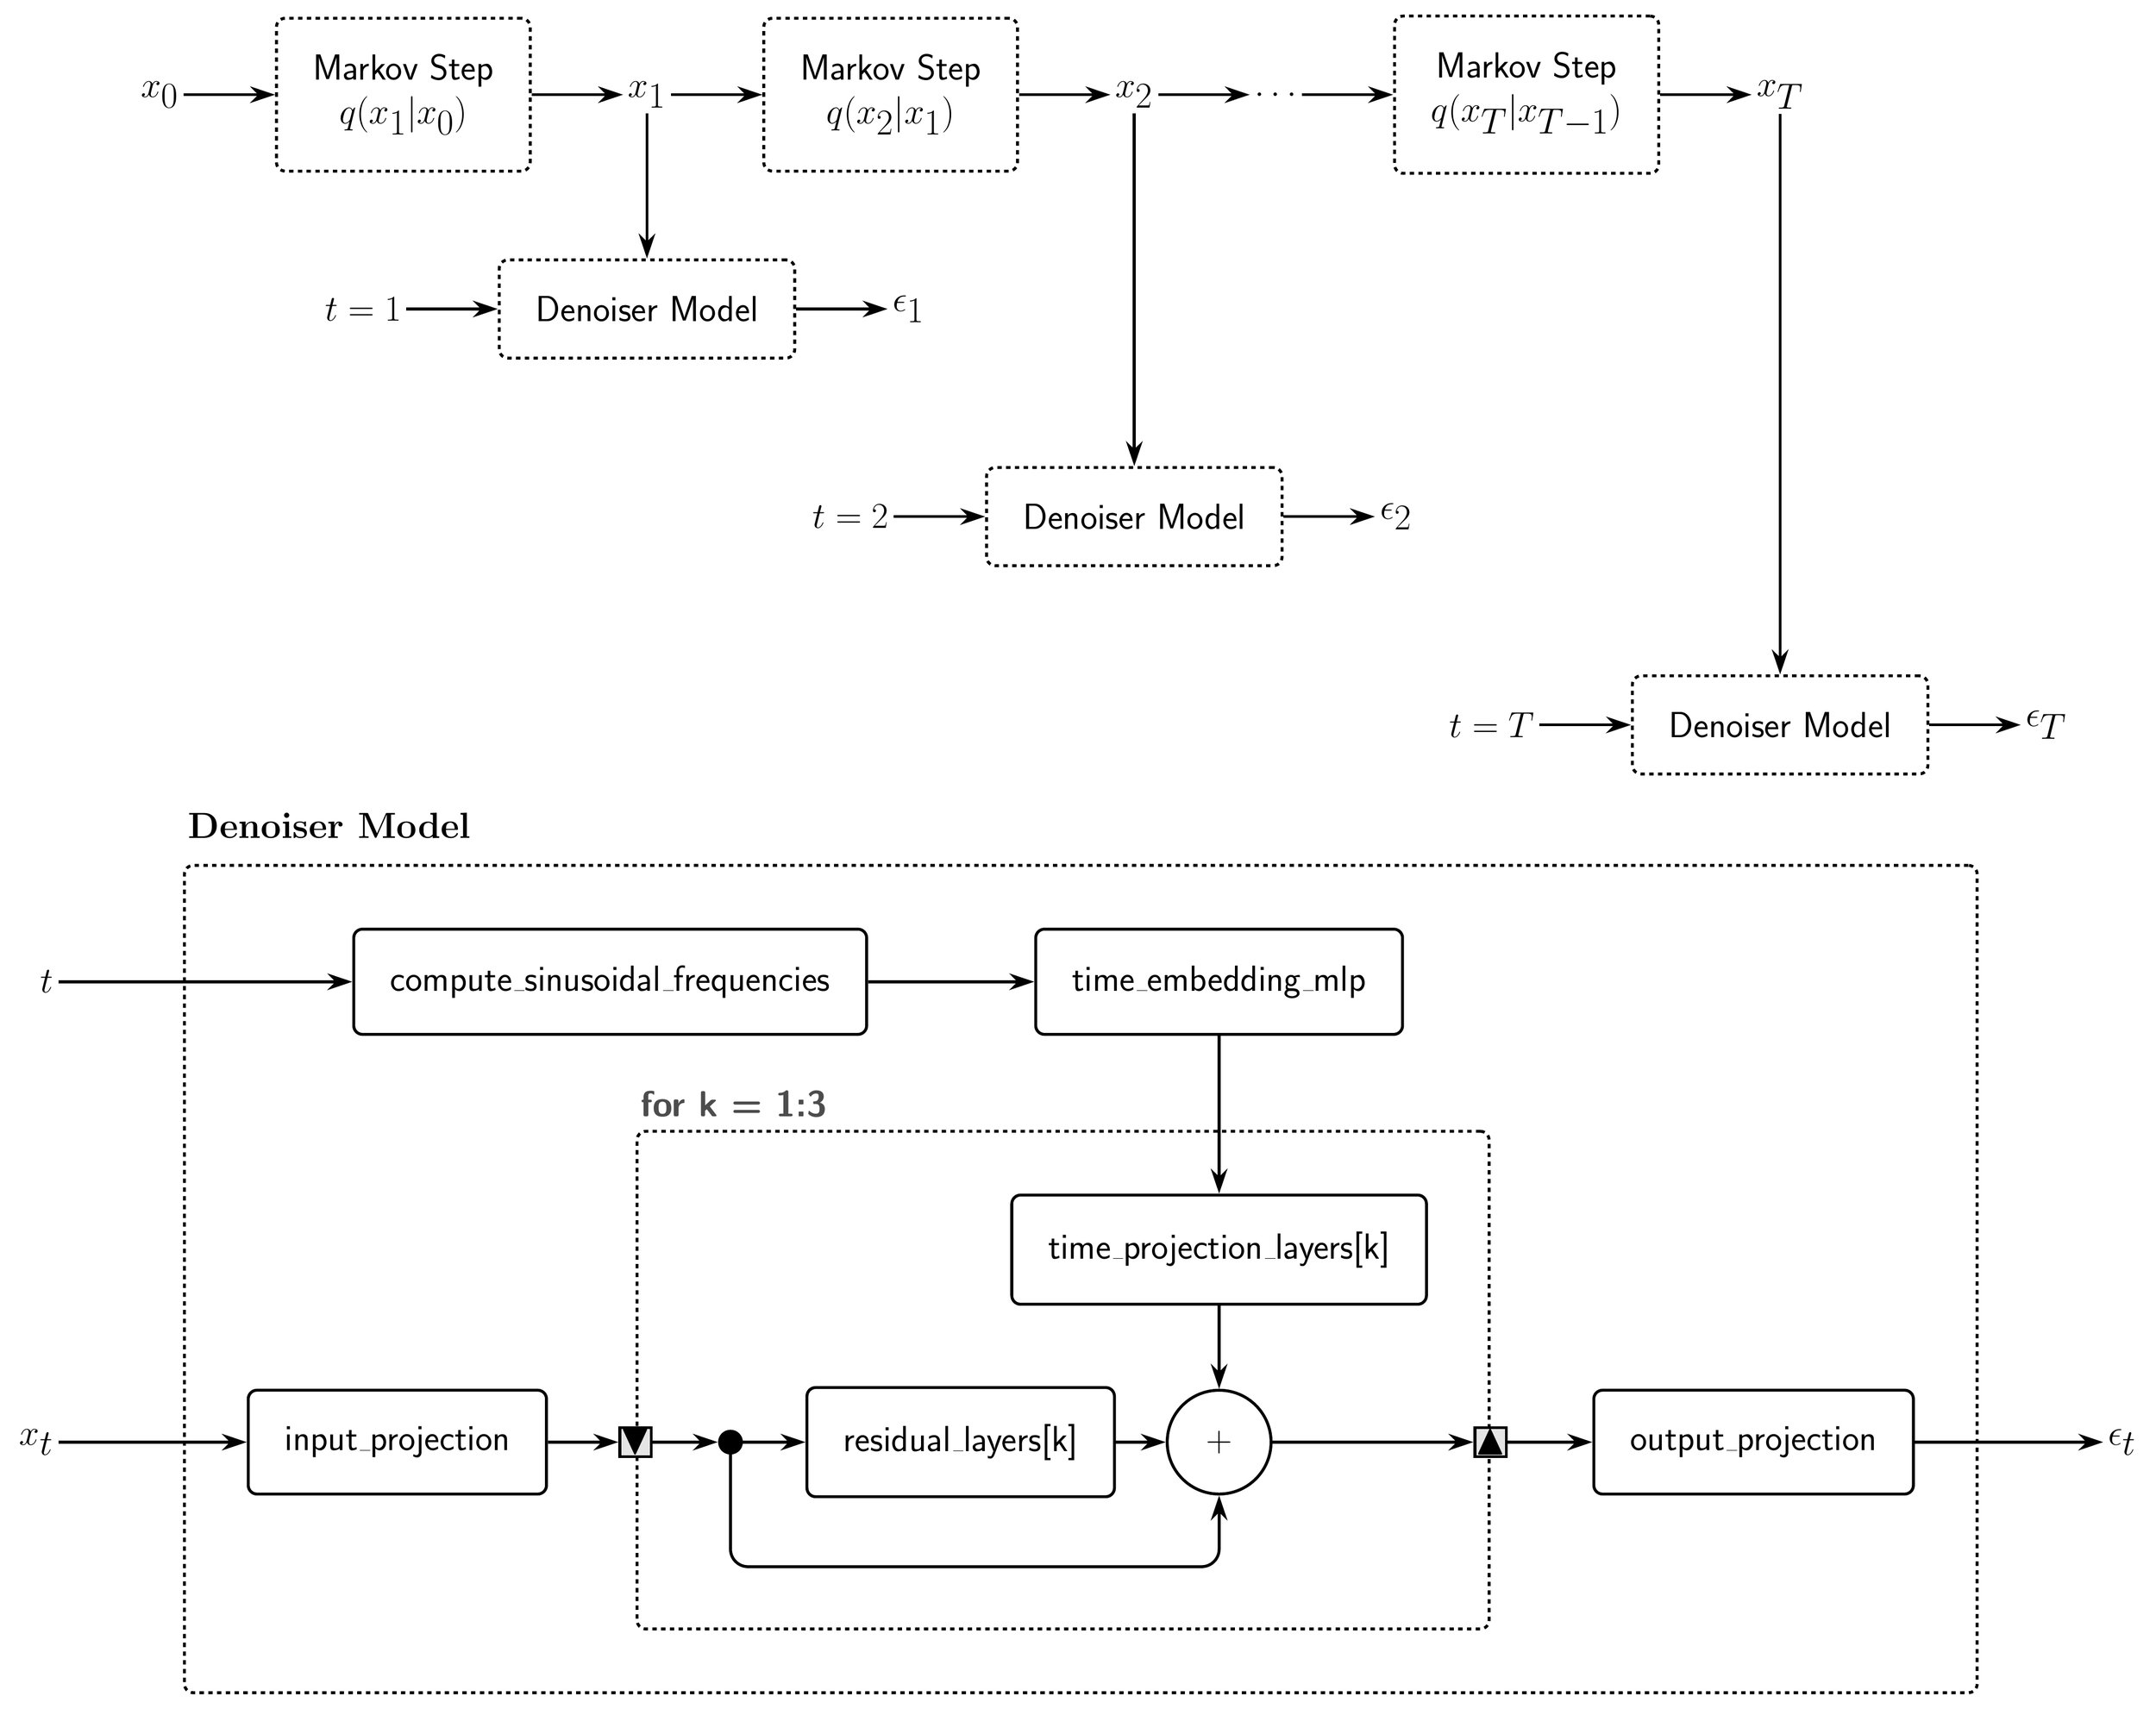
\begin{tikzpicture}[
		>={Stealth[length=6.0mm, width=4.0mm]}, 
		font=\sffamily\diagramfontsize,
		execute at begin node={\diagramfontsize},
		node distance=2.2cm and 2.2cm,
		layer/.style={rectangle, draw=black, fill=white, rounded corners=6pt, inner sep=25pt, align=center, line width=2pt},
		dashed_block/.style={rectangle, draw=black, dashed, fill=white, rounded corners=6pt, inner sep=25pt, align=center, line width=2pt},
		op/.style={circle, draw=black, fill=white, minimum size=2.5cm, inner sep=0pt, line width=2pt},
		container/.style={rectangle, draw=black, dashed, rounded corners=6pt, line width=2pt},
		loop_container/.style={rectangle, draw=black, dashed, rounded corners=6pt, line width=2pt},
		sr/.style={rectangle, draw=black, fill=black!10, minimum width=0.4cm, minimum height=0.7cm, inner sep=0pt, line width=2pt, font=\fontsize{15pt}{5pt}\selectfont}
		]
		
		% ==========================================================
		% TOP DIAGRAM: LINEAR MARKOV PROCESS WITH CASCADING DOWNWARD UNITS
		% ==========================================================
		
		% Core Chain Pipeline
		\node (x0) {$x_0$};
		\node[dashed_block, right=of x0] (m1) {Markov Step \\ $q(x_1|x_0)$};
		\node[right=of m1] (x1) {$x_1$};
		
		\node[dashed_block, right=of x1] (m2) {Markov Step \\ $q(x_2|x_1)$};
		\node[right=of m2] (x2) {$x_2$};
		
		\node[right=of x2] (dots) {$\dots$};
		\node[dashed_block, right=of dots] (mt) {Markov Step \\ $q(x_T|x_{T-1})$};
		\node[right=of mt] (xt) {$x_T$};
		
		% Flow connections for main chain
		\draw[->, line width=2pt] (x0) -- (m1);
		\draw[->, line width=2pt] (m1) -- (x1);
		\draw[->, line width=2pt] (x1) -- (m2);
		\draw[->, line width=2pt] (m2) -- (x2);
		\draw[->, line width=2pt] (x2) -- (dots);
		\draw[->, line width=2pt] (dots) -- (mt);
		\draw[->, line width=2pt] (mt) -- (xt);
		
		% Downward-branching Denoiser Blocks (Cascaded)
		\node[dashed_block, below=3.5cm of x1] (denoiser1) {Denoiser Model};
		\node[dashed_block, below=8.5cm of x2] (denoiser2) {Denoiser Model};
		\node[dashed_block, below=13.5cm of xt] (denoisert) {Denoiser Model};
		
		% Time Condition Steps
		\node[left=of denoiser1] (t1) {$t = 1$};
		\node[left=of denoiser2] (t2) {$t = 2$};
		\node[left=of denoisert] (tt) {$t = T$};
		
		% Noise Predictions
		\node[right=of denoiser1] (eps1) {$\epsilon_1$};
		\node[right=of denoiser2] (eps2) {$\epsilon_2$};
		\node[right=of denoisert] (epst) {$\epsilon_T$};
		
		% Connections tracking down into each Denoiser unit
		\draw[->, line width=2pt] (x1.south) -- (denoiser1.north);
		\draw[->, line width=2pt] (t1) -- (denoiser1);
		\draw[->, line width=2pt] (denoiser1) -- (eps1);
		
		\draw[->, line width=2pt] (x2.south) -- (denoiser2.north);
		\draw[->, line width=2pt] (t2) -- (denoiser2);
		\draw[->, line width=2pt] (denoiser2) -- (eps2);
		
		\draw[->, line width=2pt] (xt.south) -- (denoisert.north);
		\draw[->, line width=2pt] (tt) -- (denoisert);
		\draw[->, line width=2pt] (denoisert) -- (epst);
		
		% ==========================================================
		% BOTTOM DIAGRAM: HORIZONTALLY CENTERED INTERNAL ARCHITECTURE
		% ==========================================================
		\coordinate (internal_origin) at ($(x0.south)!0.5!(xt.south) + (6.0, -32.0)$);
		
		% Primary layer sequence centered around the singular remaining adder node
		\node[op, at={(internal_origin)}] (add_t) {$+$};
		\node[layer, left=of add_t, xshift=1.0cm] (c1) {residual\_layers[k]};
		\node[layer, left=of c1, xshift=-4.0cm] (in_proj) {input\_projection};
		\node[layer, right=of add_t, xshift=5.5cm] (out_proj) {output\_projection};
		
		% Loop block splitting points (One knot station before feature layer)
		\node[circle, fill=black, inner sep=6pt, left=1.5cm of c1] (solid_branch) {};
		
		% Time Embedding modules
		\node[layer, above=8.5cm of add_t] (mlp) {time\_embedding\_mlp};
		\node[layer, above=2.0cm of add_t] (time_proj) {time\_projection\_layers[k]};
		
		% Sinusoidal Frequencies
		\node[layer, left=4.0cm of mlp] (freqs) 			{compute\_sinusoidal\_frequencies};
		
		% Slightly shorter anchor below the residual loop path to reduce bounding padding cleanly
		\coordinate (residual_low_anchor) at ($(solid_branch.center) + (0.0, -3.0)$);
		
		% Ordered drawing structure within the background layer scope to prevent masking
		\begin{scope}[on background layer]
			% 1. Render nested loop box with your newly defined asymmetric parameters
			\node[loop_container, 
			inner xsep-left=2.25cm, 
			inner xsep-right=6.5cm, 
			fit={($(solid_branch) + (-\innerxsepleft, 0)$) ($(add_t) + (\innerxsepright, 0)$) (c1) (time_proj) (residual_low_anchor)}, 
			inner xsep=0pt, inner ysep=1.5cm] (loop_box) {};
			
			% 2. Render outermost container wrapper second, explicitly fitting everything inside
			\node[container, fit=(in_proj) (out_proj) (mlp) (loop_box), 
			inner xsep=1.5cm, inner ysep=1.5cm] (box) {};
		\end{scope}
		
		% LabVIEW Shift Registers placed directly on the inner loop_box borders
		\node[sr, anchor=center] (sr_left) at (loop_box.west |- c1) {\HUGE $\blacktriangledown$};
		\node[sr, anchor=center] (sr_right) at (loop_box.east |- c1) {\HUGE $\blacktriangle$};
		
		% Label for the internal loop rectangle
		\node[anchor=south west, font=\sffamily\bfseries\itshape, text=black!70] 
		at ($(loop_box.north west) + (0.0, 0.2)$) {for k = 1:3};
		
		% External layout entry/exit coordinates
		\node[left=3.0cm of box.west |- c1] (block_in) {$x_t$};
		\node[right=3.0cm of box.east |- add_t] (block_out) {$\epsilon_t$};
		\node[left=3.0cm of box.west |- mlp] (t_step) {$t$};
		
		% Core data path execution (Flows completely out, straight un-interrupted paths directly into nodes)
		\draw[->, line width=2pt] (block_in) -- (in_proj);
		\draw[->, line width=2pt] (in_proj) -- (sr_left);
		\draw[->, line width=2pt] (sr_left) -- (solid_branch);
		\draw[->, line width=2pt] (solid_branch.center) -- (c1);
		\draw[->, line width=2pt] (c1) -- (add_t);
		\draw[->, line width=2pt] (add_t) -- (sr_right);
		\draw[->, line width=2pt] (sr_right) -- (out_proj);
		\draw[->, line width=2pt] (out_proj) -- (block_out);
		
		% Time data paths (Flows completely out, straight un-interrupted paths directly into nodes)
		\draw[->, line width=2pt] (t_step) -- (freqs.west);
		\draw[->, line width=2pt] (freqs) -- (mlp.west);
		\draw[->, line width=2pt] (mlp.south) -- (time_proj.north) node[pos=0.5, right] {};
		\draw[->, line width=2pt] (time_proj.south) -- (add_t.north) node[pos=0.5, right] {};
		
		% Solid Inner Residual Connection tucked cleanly inside with adjusted lower padding clearance
		\draw[->, line width=2pt, rounded corners=12pt] (solid_branch.center) -- ++(0,-3.0) -| (add_t.south);
		
		% Title string for the outermost diagram container
		\node[anchor=south west, font=\bfseries] at ($(box.north west) + (0.0, 0.5)$) {Denoiser Model};
		
	\end{tikzpicture}
\end{document}
